\chapter{Spektroskopi Elektronik dan Fotofisika}\label{ch:b3:electronic-spectroscopy}

Di bawah lampu ultraviolet sebuah bar yang gelap, segelas air tonik
berpendar biru pucat seperti hantu. Kinina yang dikandungnya menyerap cahaya
ultraviolet, yang tidak dapat dilihat mata, lalu mengembalikan sebagiannya
beberapa nanodetik kemudian sebagai cahaya biru yang tampak. Serapan, hidup
singkat dalam keadaan tereksitasi, emisi pada panjang gelombang yang lebih
panjang, energi yang tidak kembali sebagai cahaya: nasib molekul yang
tereksitasi adalah persaingan antara proses-proses yang mempunyai tetapan
laju, dan spektrumnya dibentuk oleh vibrasi molekul itu dan oleh aturan
simetri \cref{ch:b3:group-theory-applied}. Bab ini mempelajari transisi
elektronik dan apa yang terjadi sesudahnya, yaitu bidang yang disebut
fotofisika; \cref{ch:b3:photochemistry} menambahkan kasus-kasus ketika
molekul yang tereksitasi itu bereaksi.

\begin{recall}
Jilid Tahun 1 mengukur absorbans dengan hukum Beer--Lambert,
$A =
\varepsilon\ell c$, mendefinisikan koefisien absorpsi molar, kromofor,
dan sistem terkonjugasi, serta mengaitkan warna dengan maksimum serapan. Jilid
Tahun 2 menamai orbital-orbital perbatasan HOMO dan LUMO.
\Cref{ch:b3:many-electron-atoms} mendefinisikan \omterm{def:b3:many-electron-atoms:singlet-triplet}{keadaan singlet} dan triplet;
\cref{ch:b3:group-theory-applied} teorema integral yang lenyap;
\cref{ch:b3:rovibrational-spectroscopy} tingkat-tingkat vibrasi sebuah ikatan.
\end{recall}

\begin{omfigure}
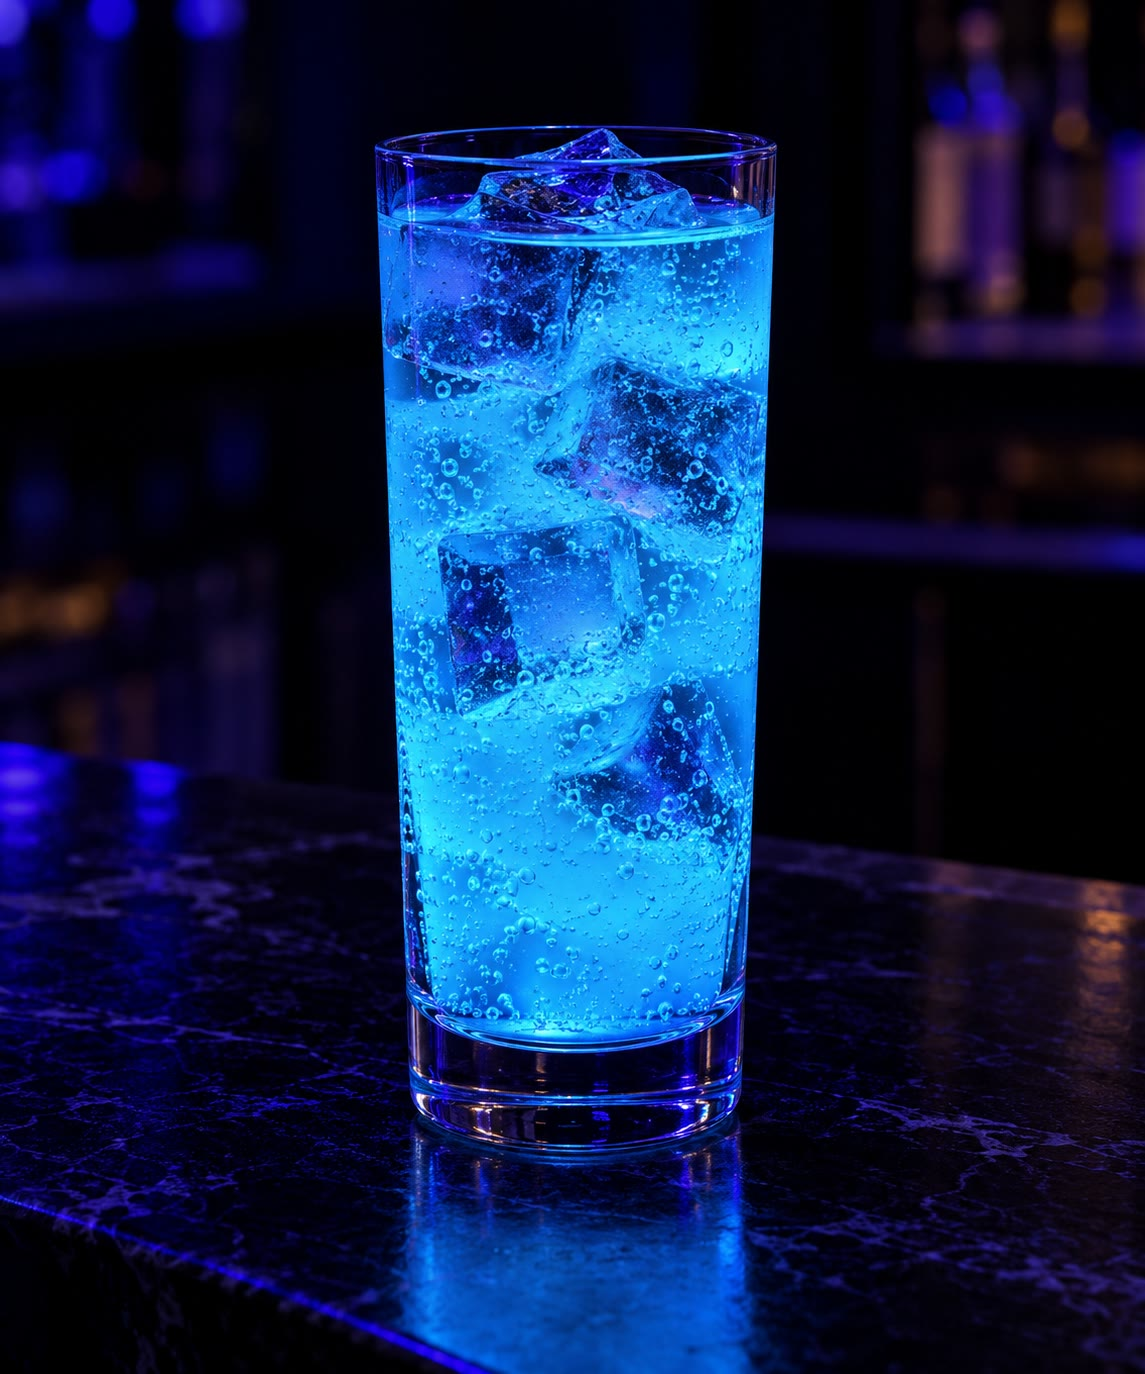
\includegraphics[height=4.6cm]{images/book4/ai/b3-07-tonic.jpg}\hspace{1em}%
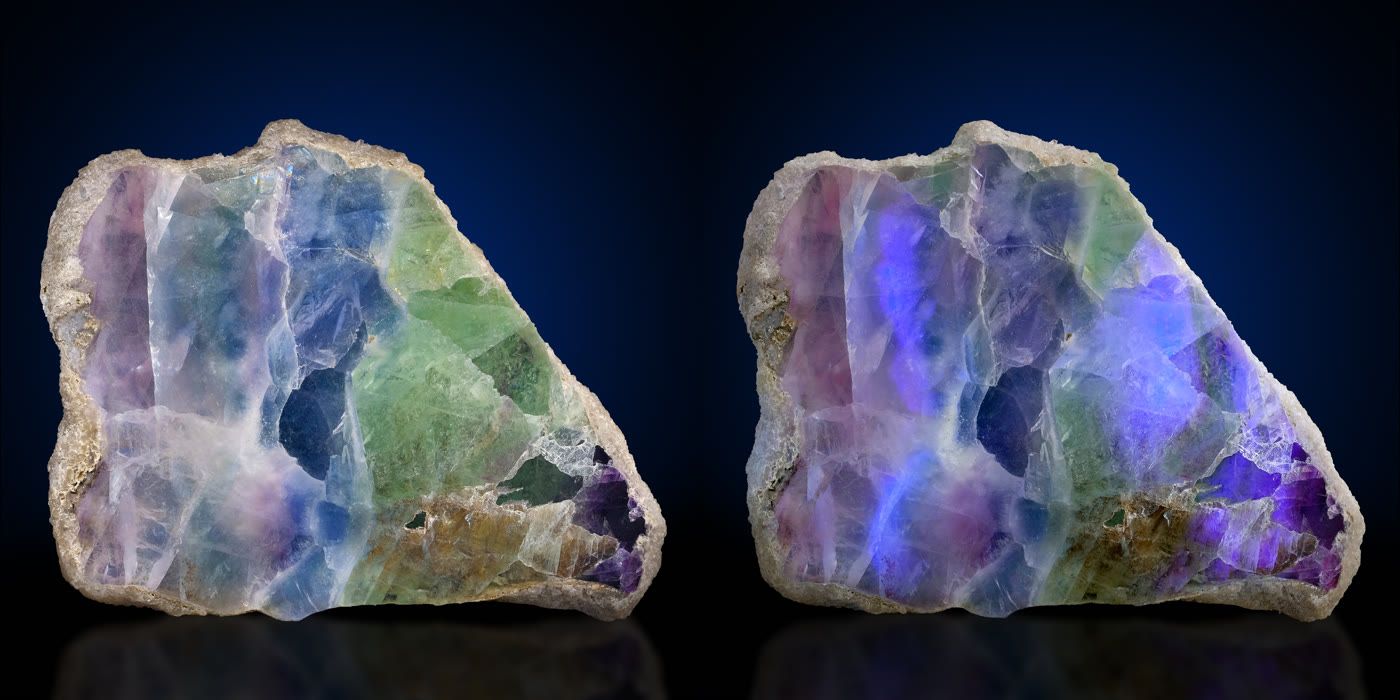
\includegraphics[height=4.6cm]{images/book4/fluorite-uv.jpg}

{\small Kiri: air tonik yang berpendar biru di bawah lampu ultraviolet.
Kanan: fluorit di bawah cahaya siang dan berfluoresensi di bawah cahaya
ultraviolet; mineral inilah yang memberi nama pada \omterm{def:b3:electronic-spectroscopy:luminescence}{fluoresensi}. Foto Masha
Milshina, CC\ BY\ 4.0.}
\end{omfigure}

\section{Transisi elektronik dan aturan seleksinya}

\begin{definition}[Momen dipol transisi, kekuatan osilator]\label{def:b3:electronic-spectroscopy:transition-dipole}
Yang disebut \emph{momen dipol transisi}\index{momen dipol transisi} antara
keadaan $\Psi_i$ dan $\Psi_f$ adalah $\boldsymbol\mu_{fi} = \langle\Psi_f|\hat{\boldsymbol\mu}|\Psi_i
\rangle$, dengan $\hat{\boldsymbol\mu} = -e\sum_k\mathbf r_k$ (ditambah muatan-muatan
inti, yang saling meniadakan di antara keadaan-keadaan yang ortogonal). Yang
disebut \emph{kekuatan osilator}\index{kekuatan osilator} $f$ adalah ukuran
tak berdimensi intensitas sebuah pita, sekitar 1 untuk transisi-transisi
yang paling kuat.
\end{definition}

\begin{proposition}[Intensitas dan kekuatan osilator]\label{prop:b3:electronic-spectroscopy:intensity}
Serapan terintegrasi sebuah pita sebanding dengan $|\boldsymbol\mu_{fi}|^2$,
dan dalam praktik
\[
f \approx 4.32\times10^{-9}\int\varepsilon(\tilde\nu)\,\dd\tilde\nu,
\]
dengan $\varepsilon$ dalam \unit{L.mol^{-1}.cm^{-1}} dan $\tilde\nu$ dalam \unit{cm^{-1}}.
\end{proposition}
\admitted

Kesebandingan itu berasal dari teori gangguan yang bergantung waktu, dan
faktor numeriknya dari osilator klasik; keduanya dibahas dalam kuliah yang
lebih lanjut. Yang penting di sini adalah bahwa $f$ hanya besar jika
$\boldsymbol\mu_{fi}$ besar, dan bahwa simetri dapat memaksanya menjadi nol.

\begin{theorem}[Aturan seleksi spin]\label{thm:b3:electronic-spectroscopy:spin-rule}
Transisi dipol listrik antara keadaan-keadaan dengan spin total yang berbeda
terlarang: $\Delta S = 0$.
\end{theorem}

\begin{proof}
Setiap keadaan adalah hasil kali sebuah fungsi ruang dan sebuah fungsi spin,
$\Psi = \phi\,\chi$. \omterm{def:b3:quantum-model-systems:operator}{Operator} dipol hanya bekerja pada posisi, sehingga
$\langle\phi_f\chi_f|\hat{\boldsymbol\mu}|
\phi_i\chi_i\rangle = \langle\phi_f|\hat{\boldsymbol\mu}|\phi_i\rangle\langle\chi_f|\chi_i\rangle$.
Fungsi-fungsi spin dengan $S$ yang berbeda adalah \omterm{def:b3:quantum-model-systems:operator}{fungsi eigen} $\hat S^2$
dengan \omterm{def:b3:quantum-model-systems:operator}{nilai eigen} yang berbeda, sehingga saling ortogonal
(\cref{thm:b3:quantum-model-systems:hermitian-real}): faktor kedua lenyap.
\end{proof}

\begin{theorem}[Aturan Laporte]\label{thm:b3:electronic-spectroscopy:laporte}
Dalam molekul yang mempunyai \omterm{def:b3:point-groups:inversion}{pusat inversi}, transisi dipol listrik harus
mengubah paritas: $g \leftrightarrow u$ diizinkan, $g \leftrightarrow g$ dan $u
\leftrightarrow u$ terlarang. Inilah \emph{aturan Laporte}\index{aturan Laporte}.
\end{theorem}

\begin{proof}
Komponen-komponen $\hat{\boldsymbol\mu}$ berganti tanda oleh inversi: komponen
itu bersifat $u$. Hasil kali $\Gamma_f\otimes\Gamma_\mu\otimes\Gamma_i$ hanya bersifat
$g$ jika $\Gamma_f$ dan $\Gamma_i$ mempunyai paritas yang berlawanan; jika tidak,
hasil kali itu bersifat $u$ dan tidak dapat memuat \omterm{def:b3:group-theory-applied:reducible}{representasi simetris total}
(\cref{thm:b3:group-theory-applied:vanishing-integral}).
\end{proof}

Kedua aturan itu ketat untuk keadaan-keadaan yang diidealkan; molekul nyata
melonggarkannya --- \omterm{def:b3:many-electron-atoms:spin-orbit}{kopling spin--orbit} mencampurkan sifat singlet dan triplet,
vibrasi menghilangkan pusat simetri untuk sesaat --- sehingga transisi-transisi
yang ``terlarang'' muncul, dengan lemah. Pita $d$--$d$ kompleks oktahedral,
yang terlarang Laporte dan lemah, mendapatkan warnanya dari pelonggaran ini
(\cref{ch:b3:complex-spectra-magnetism}).

\begin{definition}[Transisi transfer muatan]\label{def:b3:electronic-spectroscopy:charge-transfer}
Yang disebut \emph{transisi transfer muatan}\index{transisi transfer muatan}
adalah transisi yang memindahkan sebuah elektron dari orbital yang terutama
terletak pada satu bagian sistem (donor) ke orbital yang terutama terletak
pada bagian lain (akseptor); dipol transisinya besar, pitanya kuat dan lebar,
dan energinya peka terhadap kepolaran pelarut.
\end{definition}

\begin{method}[Menetapkan sebuah pita serapan]\label{met:b3:electronic-spectroscopy:assign-band}
\begin{enumerate}
  \item $\varepsilon_{\max}$ di atas sekitar \qty{e4}{L.mol^{-1}.cm^{-1}}: transisi
        yang diizinkan ($\pi\to\pi^*$ sistem terkonjugasi, atau transfer muatan).
  \item $\varepsilon_{\max}$ antara 10 dan beberapa ratus: transisi terlarang
        ($n\to\pi^*$, terlarang simetri; $d$--$d$, terlarang Laporte).
  \item $\varepsilon_{\max}$ di bawah 1: terlarang spin.
  \item Pita $n\to\pi^*$ bergeser ke panjang gelombang yang lebih pendek dalam
        pelarut protik (pasangan elektron bebasnya distabilkan oleh ikatan
        hidrogen), sedangkan pita $\pi\to\pi^*$ biasanya ke panjang gelombang
        yang lebih panjang.
\end{enumerate}
\end{method}

\section{Prinsip Franck--Condon}

\begin{theorem}[Prinsip Franck--Condon]\label{thm:b3:electronic-spectroscopy:franck-condon}
Dalam \omterm{def:b3:computational-chemistry:born-oppenheimer}{pendekatan Born--Oppenheimer}, dan jika dipol transisinya hanya sedikit
bergantung pada posisi inti, intensitas \omterm{def:b3:electronic-spectroscopy:vibronic}{transisi vibronik} dari tingkat
vibrasi $v''$ keadaan elektronik bawah ke tingkat $v'$ keadaan atas sebanding
dengan $|\langle\chi_{v'}|\chi_{v''}\rangle|^2$, yaitu kuadrat tumpang-tindih kedua
fungsi gelombang vibrasi: inilah \emph{prinsip
Franck--Condon}\index{prinsip Franck--Condon}. Transisi elektronik bersifat
vertikal: inti-inti tidak bergerak selama elektron meloncat.
\end{theorem}

\begin{proof}
Dengan $\Psi = \psi_{\mathrm{el}}(\mathbf r;R)\chi_v(R)$, momen transisinya adalah
$\int\chi_{v'}^*\big[\int\psi'^*_{\mathrm{el}}\hat\mu\psi''_{\mathrm{el}}\dd\mathbf r\big]
\chi_{v''}\,\dd R$. Suku dalam kurung siku adalah momen transisi elektronik
$\mu_{\mathrm{el}}(R)$; jika dianggap tetap (pendekatan Condon), suku itu keluar
dari integral, sehingga tersisa $\mu_{\mathrm{el}}\langle\chi_{v'}|\chi_{v''}\rangle$.
\end{proof}

\begin{definition}[Transisi vibronik, progresi, faktor Franck--Condon]\label{def:b3:electronic-spectroscopy:vibronic}
Yang disebut \emph{transisi vibronik}\index{transisi vibronik} adalah
transisi yang mengubah keadaan elektronik dan keadaan vibrasi bersama-sama;
garis-garis $v' \leftarrow 0$ untuk $v' = 0, 1, 2,
\dots$ membentuk sebuah \emph{progresi vibronik}\index{progresi vibronik};
\emph{faktor Franck--Condon}\index{faktor Franck--Condon} sebuah garis
vibronik adalah $|\langle\chi_{v'}|\chi_{v''}\rangle|^2$.
\end{definition}

\begin{proposition}[Osilator-osilator tergeser]\label{prop:b3:electronic-spectroscopy:displaced}
Jika kedua keadaan harmonik dengan frekuensi yang sama dan minimum keadaan
atas tergeser sebesar $\Delta$ (dalam satuan $\sqrt{\hbar/m\omega}$), \omterm{def:b3:electronic-spectroscopy:vibronic}{faktor-faktor
Franck--Condon} dari $v'' = 0$ membentuk distribusi Poisson,
$|\langle v'|0\rangle|^2 = \eu^{-S}S^{v'}/v'!$, dengan $S = \Delta^2/2$; garis
terkuatnya berada di dekat $v' = S$.
\end{proposition}
\admitted

Bukti umumnya memakai \omterm{def:b3:quantum-model-systems:ladder}{operator tangga} \cref{ch:b3:quantum-model-systems};
data gambar bab ini memeriksa rumus itu terhadap integrasi langsung.
Pergeseran yang kecil memberikan satu garis 0--0 yang kuat; pergeseran yang
besar memberikan progresi panjang yang anggota terkuatnya jauh dari garis
0--0.

\begin{omfigure}
\begin{tikzpicture}
\begin{axis}[name=pc, width=0.46\linewidth, height=6cm, xmin=-4, xmax=5, ymin=0,
  ymax=14, axis lines=left, xtick=\empty, ytick=\empty, xlabel={koordinat inti},
  ylabel={energi}, label style={font=\small}]
\addplot[black, thick] table[x=y, y=ground] {figdata/out/bachelor-3-franck-condon-curves.dat};
\addplot[omDef, thick] table[x=y, y=excited] {figdata/out/bachelor-3-franck-condon-curves.dat};
\draw[omabs] (axis cs:0,0.5) -- (axis cs:0,10.6);
\draw[omvib] (axis cs:-1,0.5) -- (axis cs:1,0.5);
\draw[omvib] (axis cs:0.732,9.5) -- (axis cs:2.732,9.5);
\draw[omvib] (axis cs:-0.000,10.5) -- (axis cs:3.464,10.5);
\draw[omvib] (axis cs:-0.504,11.5) -- (axis cs:3.968,11.5);
\draw[omvib] (axis cs:-0.914,12.5) -- (axis cs:4.378,12.5);
\node[font=\small, anchor=west] at (axis cs:-3.9,13.0) {tereksitasi};
\node[font=\small, anchor=west] at (axis cs:3.0,1.5) {dasar};
\node[font=\scriptsize, anchor=east] at (axis cs:-0.05,5.5) {vertikal};
\end{axis}
\begin{axis}[at={(pc.east)}, anchor=west, xshift=1.3cm, width=0.46\linewidth,
  height=6cm, xmin=-0.5, xmax=12.5, ymin=0, ymax=0.8, axis lines=left, ycomb,
  xlabel={$v'$}, ylabel={faktor Franck--Condon}, label style={font=\small},
  tick label style={font=\small}]
\addplot[black, very thick] table[x=v, y=s03] {figdata/out/bachelor-3-franck-condon-sticks.dat};
\addplot[omDef, very thick, xshift=2pt] table[x=v, y=s15] {figdata/out/bachelor-3-franck-condon-sticks.dat};
\addplot[omThm, very thick, xshift=4pt] table[x=v, y=s5] {figdata/out/bachelor-3-franck-condon-sticks.dat};
\end{axis}
\end{tikzpicture}

{\small Kiri: transisi vertikal dari tingkat terendah keadaan dasar mendarat
di tempat kurva keadaan tereksitasi, yang tergeser ke panjang ikatan yang lebih
besar, berada jauh di atas minimumnya (digambar untuk $S = 1.5$). Kanan:
\omterm{def:b3:electronic-spectroscopy:vibronic}{faktor-faktor Franck--Condon} progresi untuk $S = 0.3$ (hitam), 1.5 (biru) dan
5 (merah); setiap himpunan berjumlah 1.}
\end{omfigure}

\begin{example}[Iodin]\label{ex:b3:electronic-spectroscopy:iodine}
% ledger: diat:I2.re, diat:I2B.re, diat:I2B.we, imass:I127
Uap iodin berwarna ungu karena pita B$\leftarrow$X iodin menyerap cahaya
kuning-hijau. Ikatannya memanjang dari \qty{266.6}{pm} pada keadaan dasar
menjadi \qty{302.5}{pm} pada keadaan B. Dalam model osilator tergeser dengan
frekuensi keadaan B (\qty{125.7}{cm^{-1}}), $\Delta R = \qty{35.8}{pm}$ memberikan
$S \approx 15$: serapannya berupa progresi panjang yang garis-garis terkuatnya
berakhir pada tingkat-tingkat vibrasi tinggi keadaan B, dan kelanjutannya
masuk ke kontinum disosiasi.
\end{example}

\section{Nasib keadaan tereksitasi: diagram Jablonski}

\begin{definition}[Diagram Jablonski]\label{def:b3:electronic-spectroscopy:jablonski}
Yang disebut \emph{diagram Jablonski}\index{diagram Jablonski} adalah diagram
yang memperlihatkan keadaan-keadaan elektronik sebuah molekul (singlet
$S_0, S_1, S_2, \dots$ dalam satu kolom, triplet $T_1, T_2,
\dots$ dalam kolom lain), tingkat-tingkat vibrasinya, dan proses-proses yang
menghubungkannya: proses radiatif sebagai panah lurus, proses tanpa radiasi
sebagai panah bergelombang.
\end{definition}

\begin{definition}[Proses tanpa radiasi]\label{def:b3:electronic-spectroscopy:radiationless}
Yang disebut \emph{relaksasi vibrasi}\index{relaksasi vibrasi} adalah proses
yang membawa molekul tereksitasi ke tingkat vibrasi terendah keadaan
elektroniknya melalui tumbukan, dalam orde pikodetik. Yang disebut
\emph{konversi internal}\index{konversi internal} adalah transisi tanpa
radiasi antara keadaan-keadaan dengan multiplisitas yang sama ($S_2 \to S_1$,
$S_1 \to S_0$); \emph{lintas antarsistem}\index{lintas antarsistem} adalah
transisi semacam itu antara keadaan-keadaan dengan multiplisitas yang berbeda
($S_1 \to T_1$, $T_1 \to S_0$).
\end{definition}

\begin{definition}[Luminesensi, fluoresensi, fosforesensi, pergeseran Stokes]\label{def:b3:electronic-spectroscopy:luminescence}
Yang disebut \emph{luminesensi}\index{luminesensi} adalah pemancaran cahaya
oleh molekul yang tereksitasi. Yang disebut \emph{fluoresensi}\index{fluoresensi}
adalah emisi yang diizinkan spin, biasanya $S_1 \to S_0$, yang cepat
(nanodetik); \emph{fosforesensi}\index{fosforesensi} adalah emisi yang
terlarang spin, biasanya $T_1 \to S_0$, yang lambat (milidetik sampai
detik). Yang disebut \emph{pergeseran Stokes}\index{pergeseran Stokes} adalah
selisih antara maksimum serapan dan maksimum emisi, dinyatakan dalam energi.
\end{definition}

\begin{omfigure}
\begin{tikzpicture}[font=\small, >=Stealth]
  \foreach \y/\l in {0/{$S_0$}, 3.4/{$S_1$}, 5.6/{$S_2$}}{
    \draw[omstate] (0,\y) -- (3.6,\y); \node[anchor=east] at (-0.1,\y) {\l};
    \foreach \d in {0.25,0.5,0.75}{\draw[omvib] (0,\y+\d) -- (3.6,\y+\d);}}
  \draw[omstate] (5.0,2.5) -- (7.6,2.5); \node[anchor=west] at (7.7,2.5) {$T_1$};
  \foreach \d in {0.25,0.5,0.75}{\draw[omvib] (5.0,2.5+\d) -- (7.6,2.5+\d);}
  \draw[omabs] (0.3,0) -- (0.3,4.15) node[pos=0.35, left, font=\scriptsize, align=right] {serapan};
  \draw[omabs] (0.7,0) -- (0.7,5.85);
  \draw[omnonrad] (1.05,5.85) -- (1.05,5.6);
  \draw[omnonrad] (1.05,5.6) -- (1.05,3.4) node[pos=0.5, right, font=\scriptsize] {IC};
  \draw[omnonrad] (0.45,4.15) -- (0.45,3.42);
  \draw[omfluo] (1.7,3.4) -- (1.7,0.5) node[pos=0.5, right, font=\scriptsize, align=left] {fluor-\\esensi};
  \draw[omnonrad] (3.2,3.4) -- (3.2,0.02) node[pos=0.5, right, font=\scriptsize] {IC};
  \draw[omisc] (3.6,3.4) -- (5.0,3.1) node[pos=0.5, above, font=\scriptsize] {ISC};
  \draw[omnonrad] (5.3,3.1) -- (5.3,2.52);
  \draw[omphos] (6.0,2.5) -- (6.0,0.5) node[pos=0.5, right, font=\scriptsize, align=left] {fosfor-\\esensi};
  \draw[omisc] (5.6,2.5) -- (3.7,0.02) node[pos=0.45, above left, font=\scriptsize, inner sep=1pt] {ISC};
  \draw[omvib, dashed] (3.6,0.5) -- (6.0,0.5);
  \draw[omvib, dashed] (3.6,0.0) -- (7.6,0.0);
\end{tikzpicture}

{\small \omterm{def:b3:electronic-spectroscopy:jablonski}{Diagram Jablonski}. Panah lurus: serapan (biru), \omterm{def:b3:electronic-spectroscopy:luminescence}{fluoresensi} (merah),
\omterm{def:b3:electronic-spectroscopy:luminescence}{fosforesensi} (jingga); panah bergelombang: \omterm{def:b3:electronic-spectroscopy:radiationless}{relaksasi vibrasi} dan \omterm{def:b3:electronic-spectroscopy:radiationless}{konversi
internal} (IC); panah bergelombang putus-putus: \omterm{def:b3:electronic-spectroscopy:radiationless}{lintas antarsistem} (ISC).
Emisi berawal dari tingkat vibrasi terendah $S_1$ atau $T_1$ dan dapat
berakhir pada tingkat $S_0$ mana pun.}
\end{omfigure}

\begin{proposition}[Aturan Kasha]\label{prop:b3:electronic-spectroscopy:kasha}
\omterm{def:b3:electronic-spectroscopy:luminescence}{Luminesensi} terjadi, dengan sangat sedikit pengecualian, dari keadaan
tereksitasi terendah dengan multiplisitas tertentu ($S_1$ atau $T_1$),
keadaan mana pun yang mula-mula tereksitasi: inilah \emph{aturan
Kasha}\index{aturan Kasha}.
\end{proposition}
\begin{proof}[Kedudukan aturan ini]
Aturan ini ditetapkan secara eksperimen; alasannya adalah bahwa \omterm{def:b3:electronic-spectroscopy:radiationless}{konversi
internal} antara keadaan-keadaan tereksitasi yang lebih tinggi, yang letaknya
berdekatan, jauh lebih cepat daripada emisi, sedangkan celah $S_1$--$S_0$
besar.
\end{proof}

\begin{proposition}[Bayangan cermin]\label{prop:b3:electronic-spectroscopy:mirror}
Jika keadaan tereksitasi dan keadaan dasar mempunyai struktur vibrasi yang
serupa, pita \omterm{def:b3:electronic-spectroscopy:luminescence}{fluoresensi} adalah bayangan cermin pita serapan pertama terhadap
garis 0--0 bersama keduanya; emisinya terletak pada panjang gelombang yang
lebih panjang (\omterm{def:b3:electronic-spectroscopy:luminescence}{pergeseran Stokes}).
\end{proposition}

\begin{proof}
Serapan berlangsung dari $v'' = 0$ ke tingkat-tingkat $v'$ dari $S_1$, pada
$E_{00} + v'h\nu'$; emisi dari $v' = 0$ ke tingkat-tingkat $v''$ dari $S_0$, pada
$E_{00} - v''h\nu''$. Dengan frekuensi yang sama dan \omterm{def:b3:electronic-spectroscopy:vibronic}{faktor-faktor
Franck--Condon} yang sama (pergeseran yang sama), kedua progresi itu simetris
terhadap $E_{00}$.
\end{proof}

\begin{omfigure}
\begin{tikzpicture}
\begin{axis}[width=0.75\linewidth, height=5cm, xmin=17, xmax=33, ymin=0,
  ymax=1.15, axis x line=bottom, axis y line=left, ytick=\empty,
  xlabel={bilangan gelombang / $10^3$ cm$^{-1}$}, ylabel={intensitas},
  legend cell align=left, legend style={font=\small, draw=none, at={(0.02,0.97)}, anchor=north west},
  tick label style={font=\small}, label style={font=\small}]
\addplot[omDef, thick] table[x=nu, y=abs] {figdata/out/bachelor-3-photophysics-bands.dat};
\addlegendentry{serapan}
\addplot[omThm, thick] table[x=nu, y=em] {figdata/out/bachelor-3-photophysics-bands.dat};
\addlegendentry{fluoresensi}
\draw[gray, dashed] (axis cs:25,0) -- (axis cs:25,1.12);
\node[font=\scriptsize, gray, anchor=south west] at (axis cs:25,1.0) {0--0};
\end{axis}
\end{tikzpicture}

{\small Serapan dan \omterm{def:b3:electronic-spectroscopy:luminescence}{fluoresensi} sebuah molekul model ($S = 1$, kuantum vibrasi
\qty{1400}{cm^{-1}}): saling bayangan cermin terhadap garis 0--0; maksimum-maksimumnya
terpisah sejauh \omterm{def:b3:electronic-spectroscopy:luminescence}{pergeseran Stokes}.}
\end{omfigure}

\section{Kinetika keadaan tereksitasi}

Setelah eksitasi, populasi $S_1$ meluruh melalui setiap proses yang terbuka
baginya, masing-masing berorde satu: peluruhan radiatif $k_r$, \omterm{def:b3:electronic-spectroscopy:radiationless}{konversi
internal} $k_{\mathrm{IC}}$, \omterm{def:b3:electronic-spectroscopy:radiationless}{lintas antarsistem} $k_{\mathrm{ISC}}$.

\begin{definition}[Umur keadaan tereksitasi, umur radiatif]\label{def:b3:electronic-spectroscopy:lifetime}
Yang disebut \emph{umur keadaan tereksitasi}\index{umur keadaan tereksitasi}
adalah $\tau =
1/\sum k$, tetapan waktu peluruhan eksponensial populasi yang
tereksitasi. Yang disebut \emph{umur radiatif}\index{umur radiatif}
$\tau_r =
1/k_r$ adalah umur yang akan dimiliki keadaan itu jika emisi
merupakan satu-satunya nasibnya.
\end{definition}

\begin{definition}[Rendemen kuantum]\label{def:b3:electronic-spectroscopy:quantum-yield}
Yang disebut \emph{rendemen kuantum}\index{rendemen kuantum} sebuah proses
yang menyusul serapan cahaya adalah banyaknya peristiwa proses itu dibagi
banyaknya foton yang diserap. Yang disebut \emph{rendemen kuantum
fluoresensi}\index{rendemen kuantum fluoresensi} $\Phi_F$ adalah banyaknya
foton yang dipancarkan sebagai \omterm{def:b3:electronic-spectroscopy:luminescence}{fluoresensi} untuk setiap foton yang diserap.
\end{definition}

\begin{proposition}[Rendemen kuantum dan umur]\label{prop:b3:electronic-spectroscopy:quantum-yield}
$\Phi_F = k_r/(k_r + k_{\mathrm{IC}} + k_{\mathrm{ISC}}) = k_r\tau = \tau/\tau_r$; dengan
cara yang sama $\Phi_{\mathrm{ISC}} = k_{\mathrm{ISC}}\tau$, dan rendemen proses-proses
yang bersaing berjumlah 1.
\end{proposition}

\begin{proof}
$\dd[S_1]/\dd t = -(k_r + k_{\mathrm{IC}} + k_{\mathrm{ISC}})[S_1]$, sehingga
$[S_1] = [S_1]_0\eu^{-t/\tau}$. Banyaknya foton yang dipancarkan adalah
$\int_0^\infty k_r[S_1]\,\dd t = k_r\tau[S_1]_0$, dari $[S_1]_0$ molekul yang
tereksitasi. Integral yang sama dengan setiap $k$ memberikan setiap rendemen,
dan jumlahnya adalah $\tau\sum k = 1$.
\end{proof}

\begin{definition}[Pemadam fluoresensi, pemadaman dinamis dan statis]\label{def:b3:electronic-spectroscopy:quencher}
Yang disebut \emph{pemadam fluoresensi}\index{pemadam fluoresensi} adalah
spesies yang mengurangi \omterm{def:b3:electronic-spectroscopy:luminescence}{fluoresensi}. Dalam \emph{pemadaman
dinamis}\index{pemadaman dinamis}, spesies itu menonaktifkan molekul yang
tereksitasi melalui tumbukan, sehingga menambahkan laju $k_q[Q]$ dan
memperpendek umurnya; dalam \emph{pemadaman statis}\index{pemadaman statis},
spesies itu membentuk kompleks tak berfluoresensi dengan molekul keadaan
dasar, sehingga mengurangi intensitas tanpa mengubah umur molekul-molekul
yang masih memancar.
\end{definition}

\begin{theorem}[Persamaan Stern--Volmer]\label{thm:b3:electronic-spectroscopy:stern-volmer}
Untuk \omterm{def:b3:electronic-spectroscopy:quencher}{pemadaman dinamis},
\[
\frac{I_0}{I} = \frac{\tau_0}{\tau} = 1 + k_q\tau_0[Q] = 1 + K_{SV}[Q],
\]
yaitu \emph{persamaan Stern--Volmer}\index{persamaan Stern--Volmer}, dengan
$I_0$, $\tau_0$ diukur tanpa pemadam dan $K_{SV} = k_q\tau_0$.
\end{theorem}

\begin{proof}
Dengan pemadam, $\tau = 1/(k_0 + k_q[Q])$ dengan $k_0 = 1/\tau_0$, sehingga
$\tau_0/\tau = 1 +
k_q\tau_0[Q]$. Intensitasnya sebanding dengan
$\Phi_F = k_r\tau$, sehingga $I_0/I = \tau_0/\tau$.
\end{proof}

\begin{omfigure}
\begin{tikzpicture}
\begin{axis}[name=dec, width=0.5\linewidth, height=5cm, xmin=0, xmax=40, ymode=log,
  ymin=0.005, ymax=1.2, axis lines=left, xlabel={$t$ / ns}, ylabel={$I(t)/I(0)$},
  legend cell align=left, legend style={font=\scriptsize, draw=none, at={(0.98,0.98)}, anchor=north east},
  tick label style={font=\small}, label style={font=\small}]
\addplot[black, thick] table[x=t, y=q0] {figdata/out/bachelor-3-photophysics-decays.dat};
\addlegendentry{$[Q] = 0$}
\addplot[omDef, thick] table[x=t, y=q1] {figdata/out/bachelor-3-photophysics-decays.dat};
\addlegendentry{0.01 M}
\addplot[omProp, thick] table[x=t, y=q2] {figdata/out/bachelor-3-photophysics-decays.dat};
\addlegendentry{0.02 M}
\addplot[omThm, thick] table[x=t, y=q4] {figdata/out/bachelor-3-photophysics-decays.dat};
\addlegendentry{0.04 M}
\end{axis}
\begin{axis}[at={(dec.east)}, anchor=west, xshift=1.4cm, width=0.42\linewidth,
  height=5cm, xmin=0, xmax=0.045, ymin=0, ymax=3.3, axis lines=left,
  xlabel={$[Q]$ / mol L$^{-1}$}, ylabel={$I_0/I = \tau_0/\tau$},
  xticklabel style={/pgf/number format/fixed, /pgf/number format/precision=2},
  scaled x ticks=false, tick label style={font=\small}, label style={font=\small}]
\addplot[omThm, thick, mark=*] table[x=Q, y=I0I] {figdata/out/bachelor-3-photophysics-sv.dat};
\end{axis}
\end{tikzpicture}

{\small \omterm{def:b3:electronic-spectroscopy:quencher}{Pemadaman dinamis} sebuah fluorofor model ($\tau_0 = \qty{10}{ns}$, $k_q =
\qty{5e9}{L.mol^{-1}.s^{-1}}$). Kiri: peluruhan \omterm{def:b3:electronic-spectroscopy:luminescence}{fluoresensi}, berupa garis lurus
pada skala log, makin curam bila pemadamnya makin banyak. Kanan: garis
Stern--Volmer, dengan kemiringan $K_{SV} = k_q\tau_0 = \qty{50}{L/mol}$.}
\end{omfigure}

\begin{method}[Rendemen kuantum fluoresensi relatif]\label{met:b3:electronic-spectroscopy:relative-yield}
\begin{enumerate}
  \item Pilihlah standar dengan $\Phi_{\mathrm{std}}$ yang diketahui dan yang
        menyerap pada panjang gelombang eksitasi yang sama.
  \item Siapkan larutan encer ($A < 0.1$, untuk menghindari serapan ulang) dan
        rekam absorbans $A$ dan spektrum emisi terintegrasi $F$ larutan-larutan
        itu pada kondisi yang identik.
  \item $\Phi = \Phi_{\mathrm{std}}\,\dfrac{F}{F_{\mathrm{std}}}\,\dfrac{A_{\mathrm{std}}}{A}\,
        \dfrac{n^2}{n_{\mathrm{std}}^2}$, dengan faktor terakhir mengoreksi indeks bias
        pelarut-pelarutnya.
\end{enumerate}
\end{method}

\begin{method}[Menganalisis data pemadaman]\label{met:b3:electronic-spectroscopy:stern-volmer}
\begin{enumerate}
  \item Alurkan $I_0/I$ terhadap $[Q]$; garis lurus yang melalui 1 memberikan
        $K_{SV}$.
  \item Ukurlah juga umurnya: jika $\tau_0/\tau$ mengikuti garis yang sama,
        pemadamannya dinamis, dan $k_q = K_{SV}/\tau_0$; jika $\tau$ tidak
        berubah, pemadamannya statis.
  \item Bandingkan $k_q$ dengan batas difusi, sekitar
        \qty{e10}{L.mol^{-1}.s^{-1}} dalam air (\cref{ch:b3:rate-theories}):
        $k_q$ yang mendekatinya berarti hampir setiap pertemuan menghasilkan
        pemadaman.
\end{enumerate}
\end{method}

\begin{example}[Kinina dan antrasena]\label{ex:b3:electronic-spectroscopy:quinine}
% ledger: fl:quinine.labs, fl:quinine.eps, fl:quinine.phi, fl:anthracene.labs, fl:anthracene.phi
Kinina sulfat dalam asam sulfat \qty{0.5}{M} menyerap pada \qty{349}{nm} dengan
$\varepsilon =
\qty{5700}{L.mol^{-1}.cm^{-1}}$ dan berfluoresensi dengan
$\Phi_F = 0.546$, yang menjadikannya standar klasik untuk \omterm{def:b3:electronic-spectroscopy:quantum-yield}{rendemen kuantum}
relatif. Antrasena dalam sikloheksana menyerap pada \qty{356}{nm} dan
mempunyai $\Phi_F = 0.36$; sebagian besar sisa molekulnya yang tereksitasi
berpindah ke triplet.
\end{example}

\section{Penerapan}

\omterm{def:b3:electronic-spectroscopy:luminescence}{Fluoresensi} dideteksi dengan latar belakang yang gelap, sehingga fluorimetri
seratus sampai seribu kali lebih peka daripada spektroskopi serapan:
konsentrasi nanomolar senyawa berfluoresensi diukur secara rutin. Penanda
fluoresen melaporkan keadaan lingkungannya melalui panjang gelombang,
rendemen, atau umurnya (kepolaran, pH, terikatnya sebuah ion); transfer
energi antara dua fluorofor, yang hanya efisien dalam jarak beberapa
nanometer, mengukur jarak di dalam protein. Kompleks fosforesen logam-logam
berat, yang \omterm{def:b3:many-electron-atoms:spin-orbit}{kopling spin--orbitnya} membuat \omterm{def:b3:electronic-spectroscopy:radiationless}{lintas antarsistem} efisien,
memanen triplet dalam dioda pemancar cahaya pada layar-layar tampilan.

\begin{inthelab}[Pencacahan foton tunggal berkorelasi waktu]
Untuk mengukur umur dalam orde nanodetik, sampel dieksitasi oleh dioda laser
berpulsa dengan laju ulang megahertz, dan untuk setiap pulsa dicatat jeda
foton \omterm{def:b3:electronic-spectroscopy:luminescence}{fluoresensi} pertama yang terdeteksi. Setelah jutaan pulsa, histogram
jeda itu adalah kurva peluruhannya, yang darinya $\tau$ dicocokkan, dengan
respons instrumen diukur pada larutan penghambur. Sumber ultravioletnya
tertutup; operatornya bekerja dengan kacamata pelindung yang menahan panjang
gelombangnya.
\end{inthelab}

\begin{history}[Stokes, 1852]
George Gabriel Stokes melewatkan cahaya matahari melalui kaca ungu dan sebuah
prisma ke dalam larutan kinina, dan melihat cahaya biru muncul dari daerah yang
disinari sinar ultraviolet yang tak tampak: cahaya yang dipancarkan selalu
mempunyai panjang gelombang yang lebih panjang daripada cahaya yang diserap.
Ia menamai gejala itu \omterm{def:b3:electronic-spectroscopy:luminescence}{fluoresensi}, menurut mineral fluorit, yang berpendar
dengan cara yang sama.
\end{history}

\section{Latihan}

\begin{exercise}[$\star$]\label{exo:b3:electronic-spectroscopy:1}
Diizinkan atau terlarang, dan oleh aturan apa: (a) $S_0 \to T_1$ pada benzena;
(b) transisi $d$--$d$ kompleks oktahedral; (c) transisi $\pi\to\pi^*$ etena
($B_{1u} \leftarrow A_g$ dalam $D_{2h}$); (d) transisi $n\to\pi^*$ metanal
($A_2$)?
\end{exercise}

\begin{exercise}[$\star$]\label{exo:b3:electronic-spectroscopy:2}
Sebuah senyawa menyerap pada \qty{349}{nm} dan berfluoresensi dengan maksimum
pada \qty{450}{nm} (data latihan). Hitunglah \omterm{def:b3:electronic-spectroscopy:luminescence}{pergeseran Stokes} dalam
\unit{cm^{-1}} dan dalam eV.
\end{exercise}

\begin{exercise}[$\star$]\label{exo:b3:electronic-spectroscopy:3}
% ledger: fl:quinine.eps
Hitunglah absorbans pada \qty{349}{nm} larutan kinina sulfat \qty{1.0e-5}{mol/L}
dalam sel \qty{1}{cm}, dan fraksi cahaya yang diserapnya.
\end{exercise}

\begin{exercise}[$\star$]\label{exo:b3:electronic-spectroscopy:4}
Sebuah fluorofor mempunyai $\Phi_F = 0.60$ dan $\tau = \qty{4.0}{ns}$. Hitunglah
$k_r$, \omterm{def:b3:electronic-spectroscopy:lifetime}{umur radiatifnya}, dan jumlah tetapan laju nonradiatifnya.
\end{exercise}

\begin{exercise}[$\star\star$]\label{exo:b3:electronic-spectroscopy:5}
Sebuah pita berbentuk Gauss dengan $\varepsilon_{\max} = \qty{5700}{L.mol^{-1}.cm^{-1}}$
dan lebar penuh pada setengah maksimum \qty{5000}{cm^{-1}}. Perkirakan \omterm{def:b3:electronic-spectroscopy:transition-dipole}{kekuatan
osilatornya} (integral sebuah fungsi Gauss adalah $1.0645\,\varepsilon_{\max}\times$FWHM).
\end{exercise}

\begin{exercise}[$\star\star$]\label{exo:b3:electronic-spectroscopy:6}
Untuk osilator-osilator tergeser, carilah garis terkuat progresinya untuk
$S = 0.3$, 1.5 dan 5, serta rasio faktornya terhadap faktor garis 0--0.
\end{exercise}

\begin{exercise}[$\star\star$]\label{exo:b3:electronic-spectroscopy:7}
Dari $S_1$, $k_r = \qty{1.0e8}{s^{-1}}$, $k_{\mathrm{IC}} = \qty{2.0e7}{s^{-1}}$ dan $k_{\mathrm{ISC}} =
\qty{3.0e8}{s^{-1}}$. Hitunglah $\tau$, $\Phi_F$ dan $\Phi_{\mathrm{ISC}}$.
\end{exercise}

\begin{exercise}[$\star\star$]\label{exo:b3:electronic-spectroscopy:8}
% ledger: fl:quinine.phi, nD:water, nD:cyclohexane
\omterm{def:b3:electronic-spectroscopy:luminescence}{Fluoresensi} antrasena dalam sikloheksana ($A = 0.040$) berintegral 0.46 kali
\omterm{def:b3:electronic-spectroscopy:luminescence}{fluoresensi} kinina sulfat dalam asam sulfat encer ($A = 0.050$, $\Phi =
0.546$). Dengan indeks bias 1.4266 (sikloheksana) dan 1.333 (air, untuk asam
encer itu), hitunglah $\Phi_F$ antrasena.
\end{exercise}

\begin{exercise}[$\star\star$]\label{exo:b3:electronic-spectroscopy:9}
Umur sebuah fluorofor adalah 8.0, 5.6 dan \qty{4.3}{ns} pada konsentrasi
pemadam 0, 0.010 dan \qty{0.020}{mol/L}. Apakah pemadamannya dinamis? Carilah
$K_{SV}$ dan $k_q$.
\end{exercise}

\begin{exercise}[$\star\star\star$]\label{exo:b3:electronic-spectroscopy:10}
Penambahan sebuah pemadam mengurangi intensitas \omterm{def:b3:electronic-spectroscopy:luminescence}{fluoresensi} menjadi
setengahnya, sedangkan umur yang terukur tetap \qty{6.0}{ns}. Pemadaman jenis
apakah itu, dan apa artinya bagi keadaan dasar? Tuliskan hubungan antara
$I_0/I$ dan tetapan asosiasi kompleksnya.
\end{exercise}

\begin{exercise}[$\star\star\star$]\label{exo:b3:electronic-spectroscopy:11}
% ledger: fl:anthracene.phi
Antrasena dalam sikloheksana mempunyai $\Phi_F = 0.36$ dan, pada kondisi
sebuah pengukuran, $\tau = \qty{5.0}{ns}$ (data latihan). Hitunglah $\tau_r$,
dan rendemen triplet jika \omterm{def:b3:electronic-spectroscopy:radiationless}{konversi internal} dapat diabaikan. Mengapa \omterm{def:b3:electronic-spectroscopy:lifetime}{umur
radiatif} lebih panjang daripada umur yang terukur?
\end{exercise}

\begin{exercise}[$\star\star\star$]\label{exo:b3:electronic-spectroscopy:12}
Untuk dua elektron, fungsi spin singlet adalah
$\frac{1}{\sqrt2}[\alpha\beta - \beta\alpha]$ dan fungsi triplet $M_S = 0$ adalah
$\frac{1}{\sqrt2}[\alpha\beta + \beta\alpha]$. Tunjukkan bahwa keduanya ortogonal,
lalu simpulkan intensitas $T_1 \leftarrow S_0$ tanpa adanya \omterm{def:b3:many-electron-atoms:spin-orbit}{kopling
spin--orbit}.
\end{exercise}

\section{Soal: Mengapa Air Tonik Berpendar}

\begin{problem}[{Soal akhir pekan --- serapan oleh kinina, nasib keadaan
tereksitasinya, pemadaman oleh ion klorida, dan apakah setiap pertemuan
menghasilkan pemadaman}]
\label{pb:b3:electronic-spectroscopy:1}
% ledger: fl:quinine.labs, fl:quinine.eps, fl:quinine.phi, visc:H2O.25C
Kinina sulfat dalam asam sulfat \qty{0.5}{M}: maksimum serapan \qty{349}{nm},
$\varepsilon = \qty{5700}{L.mol^{-1}.cm^{-1}}$, $\Phi_F = 0.546$. Data soal:
umur \omterm{def:b3:electronic-spectroscopy:luminescence}{fluoresensi} tanpa pemadam adalah $\tau_0 = \qty{19}{ns}$; maksimum emisi
berada di sekitar \qty{450}{nm}; penambahan natrium klorida memberikan rasio
intensitas
\begin{center}\small
\begin{tabular}{lccccc}
\hline
$[\ce{Cl-}]$ / mol L$^{-1}$ & 0 & 0.010 & 0.020 & 0.040 & 0.080 \\
$I_0/I$ & 1.000 & 1.594 & 2.188 & 3.376 & 5.752 \\ \hline
\end{tabular}
\end{center}
Air pada \qty{25}{\celsius} mempunyai viskositas \qty{0.890}{mPa.s}; $R =
\qty{8.314}{J.K^{-1}.mol^{-1}}$.

\medskip\noindent\textbf{Bagian I --- Serapan.}
\begin{enumerate}[beginpenalty=10000]
  \item Hitunglah absorbans pada \qty{349}{nm} larutan \qty{1.0e-4}{mol/L}
        dalam sel \qty{1}{cm}.
  \item Berapa fraksi cahaya datang yang diserap?
  \item Apakah transisinya diizinkan? Gunakan $\varepsilon$.
  \item Berikan energi foton yang diserap dalam eV.
  \item Mengapa mata tidak melihat warna serapan pada air tonik?
  \item Mengapa larutan untuk pekerjaan \omterm{def:b3:electronic-spectroscopy:luminescence}{fluoresensi} dijaga di bawah
        $A = 0.1$?
\end{enumerate}

\medskip\noindent\textbf{Bagian II --- Keadaan tereksitasi.}
\begin{enumerate}[resume, beginpenalty=10000]
  \item Gambarlah \omterm{def:b3:electronic-spectroscopy:jablonski}{diagram Jablonski} proses-proses dari $S_1$.
  \item Hitunglah tetapan laju radiatif $k_r$ dan \omterm{def:b3:electronic-spectroscopy:lifetime}{umur radiatifnya}.
  \item Hitunglah tetapan laju nonradiatif totalnya.
  \item Hitunglah \omterm{def:b3:electronic-spectroscopy:luminescence}{pergeseran Stokes} dalam \unit{cm^{-1}}.
  \item Mengapa emisinya biru padahal serapannya berada di ultraviolet?
  \item Berapa fraksi energi yang diserap yang keluar sebagai \omterm{def:b3:electronic-spectroscopy:luminescence}{fluoresensi},
        dengan memperhitungkan energi setiap foton?
\end{enumerate}

\medskip\noindent\textbf{Bagian III --- Pemadaman oleh klorida.}
\begin{enumerate}[resume, beginpenalty=10000]
  \item Alurkan $I_0/I$ terhadap $[\ce{Cl-}]$ dan periksalah bahwa grafiknya
        linear.
  \item Tentukan $K_{SV}$ dengan kuadrat terkecil melalui kelima titik itu.
  \item Dengan menganggap pemadamannya dinamis, hitunglah $k_q$.
  \item Berapa umur yang akan terukur pada \qty{0.040}{mol/L}?
  \item Bagaimana membuktikan secara eksperimen bahwa pemadaman itu dinamis?
  \item Mengapa air tonik, yang tidak mengandung klorida, merupakan tempat
        yang baik bagi kinina untuk berpendar?
\end{enumerate}

\medskip\noindent\textbf{Bagian IV --- Setiap pertemuan?}
\begin{enumerate}[resume, beginpenalty=10000]
  \item Tetapan laju pertemuan yang dikendalikan difusi dalam pelarut
        berviskositas $\eta$ adalah $k_d \approx 8RT/3\eta$. Hitunglah nilainya
        dalam \unit{L.mol^{-1}.s^{-1}}.
  \item Bandingkan $k_q$ dan $k_d$.
  \item Berapa fraksi pertemuan yang menghasilkan pemadaman?
  \item Apakah pemadaman itu akan lebih cepat atau lebih lambat dalam pelarut
        yang lebih kental?
  \item Nyatakan hasilnya: rasio $k_q/k_d$ untuk pemadaman kinina oleh klorida.
\end{enumerate}
\end{problem}
